% Options for packages loaded elsewhere
\PassOptionsToPackage{unicode}{hyperref}
\PassOptionsToPackage{hyphens}{url}
%
\documentclass[
]{article}
\usepackage{amsmath,amssymb}
\usepackage{lmodern}
\usepackage{ifxetex,ifluatex}
\ifnum 0\ifxetex 1\fi\ifluatex 1\fi=0 % if pdftex
  \usepackage[T1]{fontenc}
  \usepackage[utf8]{inputenc}
  \usepackage{textcomp} % provide euro and other symbols
\else % if luatex or xetex
  \usepackage{unicode-math}
  \defaultfontfeatures{Scale=MatchLowercase}
  \defaultfontfeatures[\rmfamily]{Ligatures=TeX,Scale=1}
\fi
% Use upquote if available, for straight quotes in verbatim environments
\IfFileExists{upquote.sty}{\usepackage{upquote}}{}
\IfFileExists{microtype.sty}{% use microtype if available
  \usepackage[]{microtype}
  \UseMicrotypeSet[protrusion]{basicmath} % disable protrusion for tt fonts
}{}
\makeatletter
\@ifundefined{KOMAClassName}{% if non-KOMA class
  \IfFileExists{parskip.sty}{%
    \usepackage{parskip}
  }{% else
    \setlength{\parindent}{0pt}
    \setlength{\parskip}{6pt plus 2pt minus 1pt}}
}{% if KOMA class
  \KOMAoptions{parskip=half}}
\makeatother
\usepackage{xcolor}
\IfFileExists{xurl.sty}{\usepackage{xurl}}{} % add URL line breaks if available
\IfFileExists{bookmark.sty}{\usepackage{bookmark}}{\usepackage{hyperref}}
\hypersetup{
  pdftitle={The Impact of Wildfire Activity on Stream Temperature in Colorado Data to Policy 2021},
  pdfauthor={Jonathon Hirschi, University of Colorado Denver},
  hidelinks,
  pdfcreator={LaTeX via pandoc}}
\urlstyle{same} % disable monospaced font for URLs
\usepackage[margin=1in]{geometry}
\usepackage{longtable,booktabs,array}
\usepackage{calc} % for calculating minipage widths
% Correct order of tables after \paragraph or \subparagraph
\usepackage{etoolbox}
\makeatletter
\patchcmd\longtable{\par}{\if@noskipsec\mbox{}\fi\par}{}{}
\makeatother
% Allow footnotes in longtable head/foot
\IfFileExists{footnotehyper.sty}{\usepackage{footnotehyper}}{\usepackage{footnote}}
\makesavenoteenv{longtable}
\usepackage{graphicx}
\makeatletter
\def\maxwidth{\ifdim\Gin@nat@width>\linewidth\linewidth\else\Gin@nat@width\fi}
\def\maxheight{\ifdim\Gin@nat@height>\textheight\textheight\else\Gin@nat@height\fi}
\makeatother
% Scale images if necessary, so that they will not overflow the page
% margins by default, and it is still possible to overwrite the defaults
% using explicit options in \includegraphics[width, height, ...]{}
\setkeys{Gin}{width=\maxwidth,height=\maxheight,keepaspectratio}
% Set default figure placement to htbp
\makeatletter
\def\fps@figure{htbp}
\makeatother
\setlength{\emergencystretch}{3em} % prevent overfull lines
\providecommand{\tightlist}{%
  \setlength{\itemsep}{0pt}\setlength{\parskip}{0pt}}
\setcounter{secnumdepth}{-\maxdimen} % remove section numbering
\usepackage{floatrow}
\floatsetup[figure]{capposition=top}
\usepackage{booktabs}
\usepackage{longtable}
\usepackage{array}
\usepackage{multirow}
\usepackage{wrapfig}
\usepackage{float}
\usepackage{colortbl}
\usepackage{pdflscape}
\usepackage{tabu}
\usepackage{threeparttable}
\usepackage{threeparttablex}
\usepackage[normalem]{ulem}
\usepackage{makecell}
\usepackage{xcolor}
\ifluatex
  \usepackage{selnolig}  % disable illegal ligatures
\fi

\title{The Impact of Wildfire Activity on Stream Temperature in Colorado
Data to Policy 2021}
\author{Jonathon Hirschi, University of Colorado Denver}
\date{05/04/2021}

\begin{document}
\maketitle
\begin{abstract}
Stream temperature is an important environmental indicator as ecological
problems arise when streams get too warm. Wildfires can impact stream
temperatures in several ways, such as directly heating waters or
destroying vegetation that provides cooling shade. Climate change is
projected to cause increased wildfire activity, and it is important to
understand how this will affect water quality. Using streamflow data
from USGS, wildfire data from the National Interagency Fire Center, and
climate data from PRISM, we develop a regression model for seasonal
stream temperature for several locations in Colorado. We examine the
relationship between wildfire activity and stream temperature in
Colorado.
\end{abstract}

{
\setcounter{tocdepth}{2}
\tableofcontents
}
\hypertarget{introduction}{%
\section{Introduction}\label{introduction}}

Aquatic ecosystems are adapted to specific temperature ranges, and many
ecological problems arise when waters get too warm or too
cold.\footnote{USGS, ``Temperature and Water''.
  \url{https://www.usgs.gov/special-topic/water-science-school/science/temperature-and-water?qt-science_center_objects=0\#qt-science_center_objects}}
In the freshwater streams of Colorado, aquatic species such as plankton,
insects, and fish depend on very cool waters. The Greenback Cutthroat
Trout, the state fish of Colorado and a threatened species under the
Endangered Species Act, depends on waters as cold as 45 -- 55
\(^\circ\)C when spawning.\footnote{NRCS, ``Coldwater Fish Stream
  Habitat'', page 5.
  \url{https://efotg.sc.egov.usda.gov/references/public/CO/coldwaterfish.pdf}}
There are many environmental conditions that influence stream
temperature.

Wildfires can affect stream temperature in several ways. Fires can
directly heat waters, but they can also destroy riparian zones, bands of
lush vegetation that tend to line rivers and streams, which provide
cooling shade.\footnote{USFS, ``Fire and Riparian Areas''.
  \url{https://www.fs.fed.us/psw/topics/fire_science/ecosystems/riparian.shtml}}
With climate change projected to cause increased wildfire activity, it
is important to understand how this will affect water quality. The goal
of this analysis is to build an accurate regression model of seasonal
stream temperature, and investigate what effect wildfire activity.

\hypertarget{data-acquisition}{%
\section{Data Acquisition}\label{data-acquisition}}

The United States Geological Survey (USGS) operates water quality
monitoring sites across the nation which collect data on numerous
environmental variables. \footnote{USGS, ``Water-Quality Data for the
  Nation''. \url{https://waterdata.usgs.gov/nwis/qw}} USGS developed the
R package \emph{dataRetrieval} to allow researchers to easily access
water quality data.\footnote{USGS, ``Introduction to the dataRetrieval
  package''.
  \url{https://cran.r-project.org/web/packages/dataRetrieval/vignettes/dataRetrieval.html}}
Using this package, data was collected from the time period of 2000-2018
on the variables listed in Table 1. River discharge, or flow rate,
measures the total volume of water moving through the stream per second.
All things equal, a larger mass of water takes more energy to heat up.
Basin drainage area is a measure of the land area that feeds a stream
water through precipitation drainage.\footnote{USGS, ``Temperature and
  Water''.} Major river basin boundaries, geographic areas that have
connected streamflow and groundwater patterns, come from the Colorado
Department of Natural Resources.\footnote{Colorado DNR, ``GIS Data By
  Category''.
  \url{https://cdss.colorado.gov/gis-data/gis-data-by-category}} Table 2
below lists the number of unique USGS sites per major river basin. In
total, data was collected from 34 sites in 6 different river
basins.\footnote{There were no sites that met the filtering criteria
  from the Rio Grande River Basin, the only major basin in Colorado not
  included.} The observations were then averaged over the season of the
observation date. A map of the USGS sites with major river basin
boundaries can be seen in Figure 1.

\begin{longtable}[]{@{}
  >{\centering\arraybackslash}p{(\columnwidth - 2\tabcolsep) * \real{0.31}}
  >{\centering\arraybackslash}p{(\columnwidth - 2\tabcolsep) * \real{0.32}}@{}}
\caption{USGS Water Quality Variables}\tabularnewline
\toprule
Variable & Units \\
\midrule
\endfirsthead
\toprule
Variable & Units \\
\midrule
\endhead
Water Temperature & \(^\circ\)C \\
Observation Date & - \\
Discharge & \(ft^3 \slash sec\) \\
Altitude & Feet above sea level \\
Latitude & - \\
Longitude & - \\
Basin Drainage Area & Acres \\
River Basin & - \\
\bottomrule
\end{longtable}

\begin{longtable}[]{@{}
  >{\centering\arraybackslash}p{(\columnwidth - 2\tabcolsep) * \real{0.21}}
  >{\centering\arraybackslash}p{(\columnwidth - 2\tabcolsep) * \real{0.24}}@{}}
\caption{USGS Site Locations by River Basin}\tabularnewline
\toprule
Basin & Site Locations \\
\midrule
\endfirsthead
\toprule
Basin & Site Locations \\
\midrule
\endhead
Arkansas & 8 \\
Colorado & 7 \\
Gunnison & 5 \\
San Juan & 5 \\
South Platte & 2 \\
Yampa & 7 \\
Total & 34 \\
\bottomrule
\end{longtable}

\emph{Insert Figure 1}

Climate data from the PRISM Climate Group was collected using the R
package climateR.\footnote{ \url{https://prism.oregonstate.edu/}}
\footnote{The climateR package was developed by Mike Johnson of NOAA.}
The daily maximum air temperature and precipitation in millimeters was
extracted at the locations of the USGS sites over the relevant time
period. The climate data was combined with the water quality data by
location and time. Air temperature strongly influences water
temperature, and rainfall can have a warming affect on
streams.\footnote{Benyahya et. al., ``A Review of Statistical Water
  Temperature Models''. \emph{Canadian Water Resources Journal}
  September 2007: page 181.}

The National Interagency Fire Center (NIFC) provides spatial data for
the locations, dates, and sizes of wildfires in America from
2000-2018.\footnote{NIFC, ``Historic Perimeters Combined 2000-2018''.
  \url{https://data-nifc.opendata.arcgis.com/datasets/historic-perimeters-combined-2000-2018?geometry=47.717\%2C-9.831\%2C68.108\%2C74.202}}
Colorado had 953 recorded wildfires over this time period. Then, the
total number of fires and total acres burned in a season was calculated
for each major river basin. This data was then combined with the water
quality data, with year, season, and basin used to combine the data.

\hypertarget{data-exploration}{%
\section{Data Exploration}\label{data-exploration}}

In this section, several relationships between the variables are
explored visually. All variables observed over time have been combined
by year and season (and basin for wildfire data). The response variable
for modeling will be water temperature. The distribution for water
temperature can be seen in Figure 2. The range of temperatures is wide
because the observations include cold mountain streams in the winter and
warm rivers in the winter.

\emph{Insert Figure 2}

Water temperature has a strong relationship with air temperature and
season, as seen in Figure 3. Clearly, both water and air temperatures
are coolest in the winter and warmest in the summer. The relationship is
largely linear, but the relationship flattens out for lower water
temperatures. This dynamic is complicated, but it is in part due to how
very cold water resists freezing solid when it is flowing through a
channel.\footnote{Benyahya, 2007.}

\emph{Insert Figure 3}

Stream discharge is strongly related to season, as seen in Figure 4.
Flow rates are highest in the summer and lowest in the winter. The
relationship between discharge and water temperature is much less clear.
In the first plot, discharge can be seen to span several orders of
magnitude and the relationship with water temperature is not apparent.
This suggests a log transformation might be worth investigating. In
second plot, the relationship between log discharge and water
temperature is complex, partly due to repeated observations from the
same USGS sites having related discharges. There is a slight positive
relationship between log discharge and water temperature.

\emph{Insert Figure 4}

Altitude has a strong negative relationship with water temperature,
which is largely linear, as can be seen in the left plot of Figure 5.
Unsurprisingly, streams at higher altitudes have cooler water. In
Colorado, altitude is strongly related to longitude due to the relative
north to south orientation of the Rocky Mountains in the middle of the
state. In the plot on the right of Figure 5, the altitude increases to a
peak and then decreases as you move east to west. Each point in these
plots represents the overall average temperature for a single stream
monitoring site, as for the stream altitude is treated as constant
through time.

\emph{Insert Figure 5}

In the left plot of Figure 6, drainage area has a positive but nonlinear
relationship with water temperature. Additionally, drainage area spans
over several orders of magnitude. These relationships suggest a log
transformation might be useful for this variable. On the right of Figure
6, the log transformation of drainage area has a much more linear
relationship with water temperature. In these plots, each point
represents the overall average temperature for a USGS site, as drainage
area is treated as constant through time.

\emph{Insert Figure 6}

For the predictors related to wildfires, the number of wildfires in a
season is obviously related to the total number of acres burned in a
season. To avoid using both correlated predictors, the total number of
acres burned will be considered for modeling. Conceptually, the total
number of acres burned mostly captures the information found in the
total number of wildfires. The effect on the environment of two small
fires would seem to be similar to effect of one wildfire that was the
size of the two smaller ones put together. The relationship between
total acres burned in a river basin and water temperature is depicted in
Figure 7. The acres burned in a basin is strongly related to season:
there is the most wildfire activity in the summer and the least in the
winter. A log transformation might be considered for modeling because
the acres burned by wildfire spans several orders of magnitude and the
relationship with water temperature appears nonlinear.\footnote{To
  account for seasons with zero acres burned by wildfire, the log
  transformation needs to be shifted by adding one.} It is difficult to
discern, but there is a slight positive relationship between acres
burned by wildfire and water temperature.

\emph{Insert Figure 7}

Although the data contains repeated measurements at the various USGS
sites, that is ignored in this analysis. Modeling the repeated measures
is out of the scope of this project.

\hypertarget{variable-selection-and-collinearity-checks}{%
\section{Variable Selection and Collinearity
Checks}\label{variable-selection-and-collinearity-checks}}

To arrive at a set of regressors to model stream temperature, we first
examine the collinearity for the full set of predictors. The predictors
under consideration include: year, season, discharge, precipitation, air
temperature, altitude, drainage acreage, basin indicator, and acres
burned in the basin. The variance inflation factors (VIFs) are presented
below in Table 3.

\begin{longtable}[]{@{}
  >{\centering\arraybackslash}p{(\columnwidth - 2\tabcolsep) * \real{0.22}}
  >{\centering\arraybackslash}p{(\columnwidth - 2\tabcolsep) * \real{0.17}}@{}}
\caption{Full Model VIF}\tabularnewline
\toprule
Regressor & VIF.Value \\
\midrule
\endfirsthead
\toprule
Regressor & VIF.Value \\
\midrule
\endhead
Year & 1.27 \\
Season & 14.86 \\
Discharge & 2.4 \\
Precipitation & 1.42 \\
Max Air Temp & 13.58 \\
Altitude & 4.26 \\
Drainage & 3.9 \\
Basin & 3.69 \\
Acres Burned & 1.11 \\
\bottomrule
\end{longtable}

The VIF for the season predictor is roughly 14.9. As could be seen in
the exploratory plots from the previous section, many of the predictors
are related to season. Discharge, precipitation, air temperature, and
wildfire activity are all at their highest levels in the summer, and at
their lowest levels in the winter. In order to make more valid inference
on the regression parameters, the factor variable for season is
amputated from the model. The VIF values for the reduced model are
presented below in Table 4.

\begin{longtable}[]{@{}
  >{\centering\arraybackslash}p{(\columnwidth - 2\tabcolsep) * \real{0.22}}
  >{\centering\arraybackslash}p{(\columnwidth - 2\tabcolsep) * \real{0.17}}@{}}
\caption{Reduced Model VIF}\tabularnewline
\toprule
Regressor & VIF.Value \\
\midrule
\endfirsthead
\toprule
Regressor & VIF.Value \\
\midrule
\endhead
Year & 1.25 \\
Discharge & 2.2 \\
Precipitation & 1.21 \\
Max Air Temp & 1.24 \\
Altitude & 3.39 \\
Drainage & 3.81 \\
Basin & 3.4 \\
Acres Burned & 1.1 \\
\bottomrule
\end{longtable}

After removing season from the model specification, there are no
remaining regressors with VIF values over 5, which is a common heuristic
threshold for identifying correlated regressors. With collinearity
addressed, variable selection can be undertaken without large concern
for unreliable parameter estimates. Using an exhaustive model search
procedure, the Bayesian Information Criterion (BIC) is compared for the
best models of various sizes. The basin factor variable is omitted from
this step, and it will be considered for inclusion later.\footnote{The R
  function \emph{regsubsets} does not behave well with factors.
  Additionally, the BIC values calculated in that function differ from
  manually computed BIC values by a constant amount.}

\emph{Insert Figure 8}

The minimum BIC value is for the model with 6 predictors.\footnote{The
  intercept brings it to 7 total regression parameters.} The one
predictor omitted from the best model by this criterion was acres burned
by wildfire, which is the variable of primary research interest. Since
the BIC was quite similar for the model with 7 predictors (including
acres burned), the estimated out-of-sample prediction error is presented
for those two models using 10-fold cross validation in Table 5.

\begin{longtable}[]{@{}
  >{\centering\arraybackslash}p{(\columnwidth - 6\tabcolsep) * \real{0.26}}
  >{\centering\arraybackslash}p{(\columnwidth - 6\tabcolsep) * \real{0.33}}
  >{\centering\arraybackslash}p{(\columnwidth - 6\tabcolsep) * \real{0.11}}
  >{\centering\arraybackslash}p{(\columnwidth - 6\tabcolsep) * \real{0.11}}@{}}
\caption{10-Fold Cross Validation - Acres Burned
Included}\tabularnewline
\toprule
Model Predictors & Includes Acres Burned & RMSE & MAE \\
\midrule
\endfirsthead
\toprule
Model Predictors & Includes Acres Burned & RMSE & MAE \\
\midrule
\endhead
6 & No & 1.657 & 1.296 \\
7 & Yes & 1.653 & 1.293 \\
\bottomrule
\end{longtable}

The root mean squared error (RMSE) and mean absolute error (MAE) are
both slightly lower for the model including acres burned. Since the BIC
and cross-validated values are so similar for the two models, the larger
model with the variable of primary research interest will be used.
Finally, the basin factor variable is added manually, and the 10-fold
cross validation metrics are computed for that model.

\begin{longtable}[]{@{}
  >{\centering\arraybackslash}p{(\columnwidth - 6\tabcolsep) * \real{0.26}}
  >{\centering\arraybackslash}p{(\columnwidth - 6\tabcolsep) * \real{0.24}}
  >{\centering\arraybackslash}p{(\columnwidth - 6\tabcolsep) * \real{0.11}}
  >{\centering\arraybackslash}p{(\columnwidth - 6\tabcolsep) * \real{0.11}}@{}}
\caption{10-Fold Cross Validation - Basin Included}\tabularnewline
\toprule
Model Predictors & Includes Basin & RMSE & MAE \\
\midrule
\endfirsthead
\toprule
Model Predictors & Includes Basin & RMSE & MAE \\
\midrule
\endhead
7 & No & 1.653 & 1.293 \\
8 & Yes & 1.632 & 1.286 \\
\bottomrule
\end{longtable}

The RMSE and MAE are again slightly lower for the model that includes
basin, so that factor variable will be included in the model. The final
model is represented mathematically below. This model will be fit and
checked for structural issues and violations of regression assumptions.
The parameter values are represented as \(\beta\)'s, with \(\beta_0\)
corresponding to the intercept and the errors assumed to be normally
distributed with mean zero, or \(\epsilon \sim N(0, \sigma^2)\).

\[Water\,Temp. = \beta_0 + \beta_1 Year + \beta_2  Discharge + \beta_3  Precip. +\]
\[+ \beta_4 AirTemp + \beta_5 Altitude + \beta_6  DrainageArea + \beta_7 AcresBurned + \beta_8 Basin + \epsilon\]

\hypertarget{model-structure-and-assumptions}{%
\section{Model Structure and
Assumptions}\label{model-structure-and-assumptions}}

First, the model with the original, non-transformed predictors is
examined. In Figure 9, there are clear nonlinear relationships for
several predictors. An iterative procedure was used to compare log
transformations for one variable at a time, the full details of which
are omitted here. This procedure arrived on log transformations for
discharge (flow) and precipitation.\footnote{For precipitation, the same
  shift discussed earlier is applied, where 1.0 is added before the log
  transformation is applied to account for observations with zero
  precipitation.}

\emph{Insert Figure 9}

The log transformations discussed previously accounted for many of the
nonlinear relationships, as can be seen in Figure 10. Although visual
inspection of the relationship between acres burned and water
temperature was suggestive of a log transformation, the model had a
lower BIC value when this transformation was made. There is still a
nonlinear pattern for air temperature (tmax) and the Pearson residuals
versus fitted values.

\emph{Insert Figure 10}

A quadratic trend for air temperature is fit, where the square of air
temperature is added to the model. In Figure 11, there is now a linear
relationship with air temperature, and additionally the residuals versus
fitted values in the bottom right plot now have a linear relationship.

\emph{Insert Figure 11}

The model diagnostics discussed previously in this section together give
evidence that there are no major structural issues with the mean portion
of the model. Next, the model is examined for influential observations
and outliers. Observations 11 and 1,229 are identified as leverage
points by the influence index plot seen in Figure 12. However, an
outlier test with Bonferroni correction does not identify either
observation as an outlier. Observation 232 is the only observation
identified as an outlier\footnote{Bonferroni-corrected p-value of 0.01}
Finally, the influence plot seen in Figure 13 show that observations 11
and 1229 have very small residuals, and the outlier at observation 232
has relatively low influence. For these reasons, combined with the lack
of obvious structural issues in the residual plots, no observations will
be removed from the model. Furthermore, since the response variable is
average seasonal values, conceptually it would seem problematic to
identify an entire seasonal average as an outlier and remove it from the
model.

\emph{Insert Figures 12 \& 13}

In the plot of fitted values versus residuals in Figure 14, the
residuals exhibit a slight ``fan'' shape, where they are smaller in
absolute terms for lower fitted values and then increase. Also, at lower
fitted values, the residuals do not appear to be centered at zero. So
the assumptions of constant variance of errors and mean zero errors
might be violated. The plot of fitted values versus observed values is
quite linear, although the trend might flatten out slightly for lower
fitted values. There are a number of ways this model could be extended,
as will be mentioned in the discussion section. But for this version of
the analysis, no further structural changes will be made.

\emph{Insert Figure 14}

\hypertarget{results}{%
\section{Results}\label{results}}

The model fit the data quite well, with an adjusted \(R^2\) value of
roughly 0.95. For ease of interpretation, three predictors were shifted
by a constant amount: acres burned by wildfire now has units of 1,000
acres, altitude now represents hundreds of feet, and drainage area
represents hundreds of acres. The direction and relative magnitude of
the effects is displayed in Table X, along with the relative statistical
significance level.\footnote{Three stars represents s p-value of less
  than \(1\times 10^{-6}\)}

\begin{longtable}[]{@{}
  >{\centering\arraybackslash}p{(\columnwidth - 4\tabcolsep) * \real{0.33}}
  >{\centering\arraybackslash}p{(\columnwidth - 4\tabcolsep) * \real{0.28}}
  >{\centering\arraybackslash}p{(\columnwidth - 4\tabcolsep) * \real{0.38}}@{}}
\caption{Variable Effects Table}\tabularnewline
\toprule
Regressor & Effect Direction & Statistical Significance \\
\midrule
\endfirsthead
\toprule
Regressor & Effect Direction & Statistical Significance \\
\midrule
\endhead
Year & Slightly Negative & not significant \\
Log Discharge & Negative & *** \\
Log Precipitation & Strongly Positive & *** \\
Max Air Temperature - Quadratic & Strongly Positive & *** \\
Altitude & Slightly Negative & *** \\
Acres Burned & Slightly Positive & not significant \\
Drainage Area & Slightly Positive & *** \\
Basin & Mixed & Mixed \\
\bottomrule
\end{longtable}

The direction of the relationships for the statistically significant
regressors matched the theoretical relationship with water temperature.
Discharge is negatively associated with water temperature, likely
because a larger mass of water takes longer for the air to warm up.
Precipitation was positively associated with water temperature, and the
quadratic trend for air temperature was positively associated with water
temperature. Altitude was negatively associated with water temperature,
and basin drainage area was had a positive association. Over the 18 year
period of observations, there was on average a slight downward trend in
temperature, but the evidence was consistent with there being no
year-to-year trend. There were observations from six river basins, and
the effects plot for that predictor can be seen in Figure 15. The
Arkansas river basin had on average the warmest water temperatures.
Using this basin as the baseline for comparison, there were
statistically significant differences between the Colorado and San Juan
river basins,\footnote{P-values of less than \(1\times 10^{-6}\). In the
  Colorado DNR data, the San Juan river basin is grouped in with the
  Dolores river basin.} the latter of which had the coldest water
temperatures on average.

\emph{Insert Figure 15}

The main research interest was on the relationship between wildfire
activity and water temperature, and for this analysis the data was
consistent with there being no relationship. The effects plot for acres
burned can be seen in Figure 16.\footnote{As mentioned before, the units
  now represent thousands of acres.} The relationship is slightly
positive, but there is substantial variation. On the low end of the
confidence interval, there would be a slight negative relationship
between acres burned in a river basin and water temperature. This is
unlikely to be the case based off of theoretical considerations, but
wildfires can cause many physical and chemical changes in water systems,
and there could be circumstances where there is a net cooling effect.

\emph{Insert Figure 16}

\hypertarget{discussion}{%
\section{Discussion}\label{discussion}}

On the high end of the confidence interval, the effect size was
comparable in magnitude to the mean effect sizes for altitude and
drainage area,\footnote{The 97.5 percentile coefficient for effect size
  was roughly \(0.01\), compared to point estimates of \(-0.03\) and
  \(0.01\) for altitude and drainage area, respectively. Both altitude
  and drainage area were arithmetic in scale, so this comparison is
  valid.} so while the data does not tell a clear picture, the results
combined with theoretical considerations of the effects of wildfires
tells us that further research is merited on the topic.

There are many ways this analysis could be augmented. First, repeated
observations at individual USGS monitoring sites was ignored, and this
could be incorporated into a mixed effects model or some other
statistical tool. Next, finer spatial and temporal resolution could be
illuminating; river basins, while important geographic units, are very
large areas. Similarly, grouping observations by season is a very long
time span. Finally, there are more advanced spatial methods that might
be applied to the wildfire data. This analysis could serve as a valuable
first step in that more advanced research.

It is notable that the model provided a high degree of fit to the data,
with an adjusted \(R^2\) of roughly 0.95. Researchers have developed
very accurate climate forecasting models, so stream temperature models
such as the one in this analysis could be projected forward to study how
climate change might effect aquatic ecosystems in Colorado.

\hypertarget{references}{%
\section{References}\label{references}}

National Resource Conservation Service, ``Coldwater Fish Stream
Habitat'', page 5.
\url{https://efotg.sc.egov.usda.gov/references/public/CO/coldwaterfish.pdf}

United States Geological Survey, ``Temperature and Water''.
\url{https://www.usgs.gov/special-topic/water-science-school/science/temperature-and-water?qt-science_center_objects=0\#qt-science_center_objects}

United States Forest Service, ``Fire and Riparian Areas''.
\url{https://www.fs.fed.us/psw/topics/fire_science/ecosystems/riparian.shtml}

USGS, ``Water-Quality Data for the Nation''.
\url{https://waterdata.usgs.gov/nwis/qw}

USGS, ``Introduction to the dataRetrieval package''.
\url{https://cran.r-project.org/web/packages/dataRetrieval/vignettes/dataRetrieval.html}

Colorado DNR, ``GIS Data By Category''.
\url{https://cdss.colorado.gov/gis-data/gis-data-by-category}

NIFC, ``Historic Perimeters Combined 2000-2018''.
\url{https://data-nifc.opendata.arcgis.com/datasets/historic-perimeters-combined-2000-2018?geometry=47.717\%2C-9.831\%2C68.108\%2C74.202}

PRISM Climate Data, \url{https://prism.oregonstate.edu/}

Benyahya et. al., ``A Review of Statistical Water Temperature Models''.
\emph{Canadian Water Resources Journal} September 2007: page 181.

\hypertarget{appendix-a-numbered-figures}{%
\section{Appendix A: Numbered
Figures}\label{appendix-a-numbered-figures}}

\begin{figure}
\centering
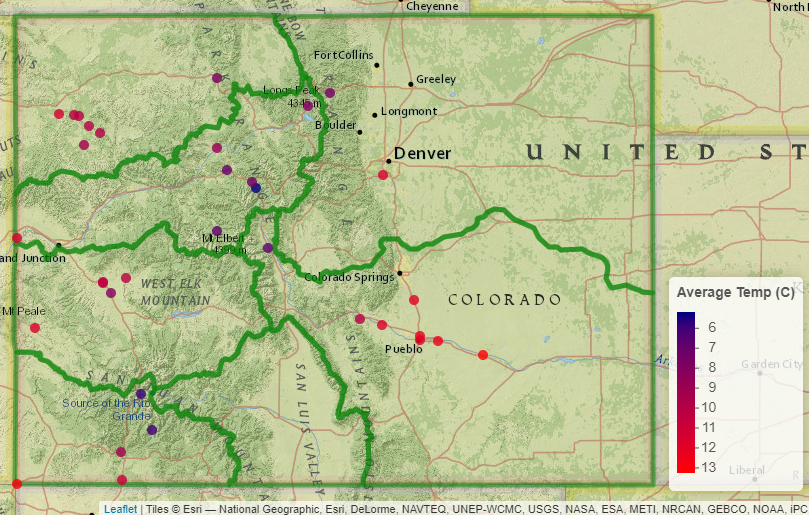
\includegraphics{D:/Projects/D2P 2021/Report/Images/site_map.png}
\caption{USGS Site Locations - With Basin Boundaries.}
\end{figure}

\begin{figure}
\centering
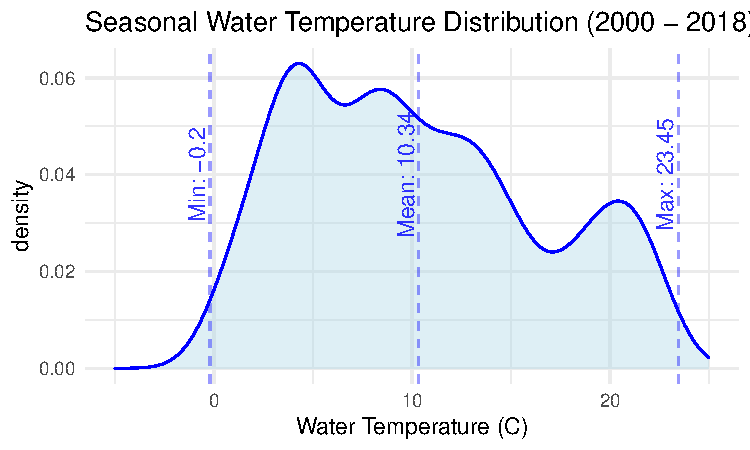
\includegraphics{D2P-Report_files/figure-latex/fig2-1.pdf}
\caption{\label{fig:figs1}Temperature Distribution}
\end{figure}

\begin{figure}
\centering
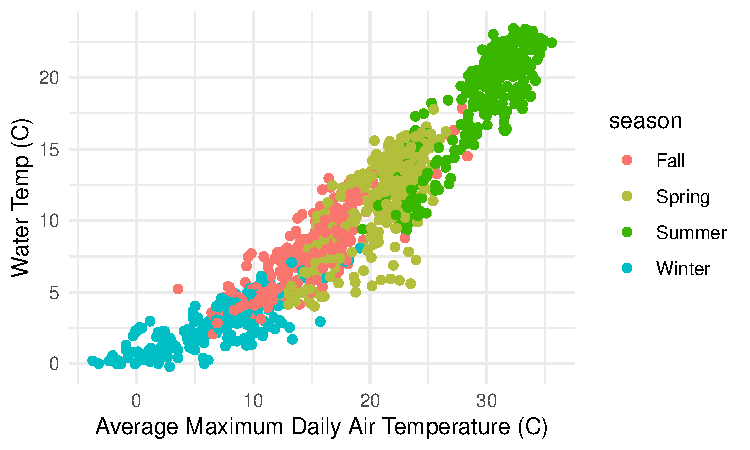
\includegraphics{D2P-Report_files/figure-latex/fig3-1.pdf}
\caption{\label{fig:figs3}Air Temperature versus Water Temperature}
\end{figure}

\begin{figure}
\centering
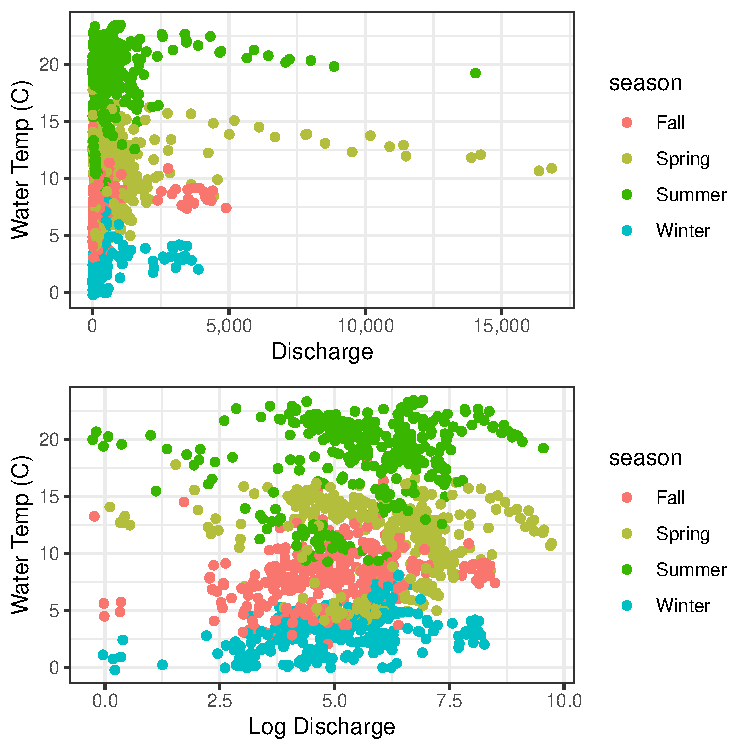
\includegraphics{D2P-Report_files/figure-latex/fig4-1.pdf}
\caption{\label{fig:figs4}Log Discharge versus Water Temperature}
\end{figure}

\begin{figure}
\centering
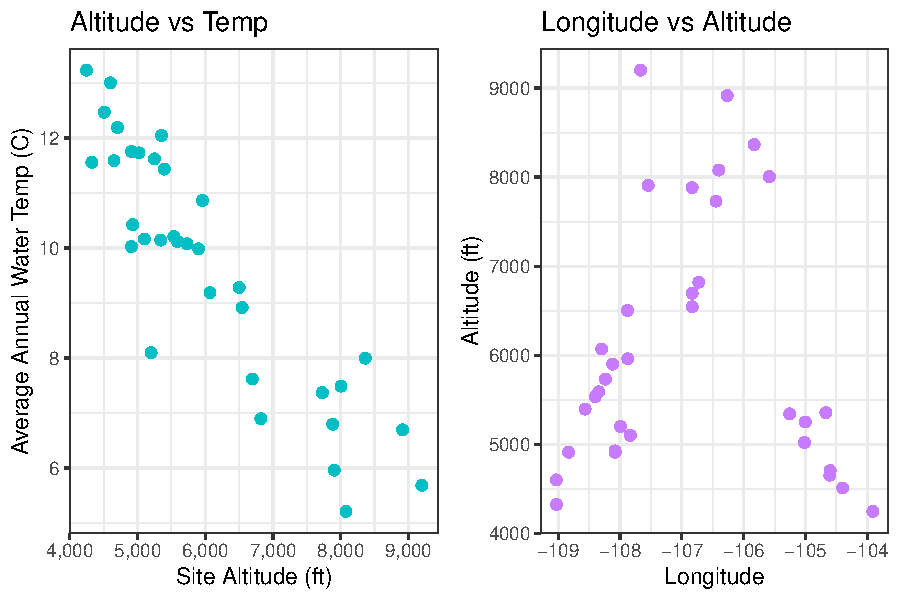
\includegraphics{D2P-Report_files/figure-latex/fig5-1.pdf}
\caption{\label{fig:figs5}Altitude, Longitude, and Water Temperature}
\end{figure}

\begin{figure}
\centering
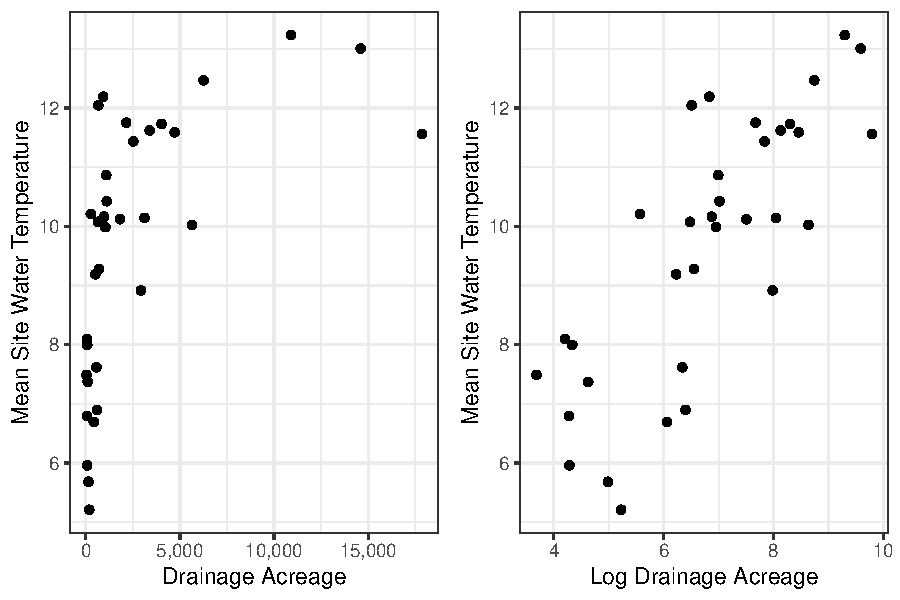
\includegraphics{D2P-Report_files/figure-latex/fig6-1.pdf}
\caption{\label{fig:figs6}Drainage Area and Average Water Temperature}
\end{figure}

\begin{figure}
\centering
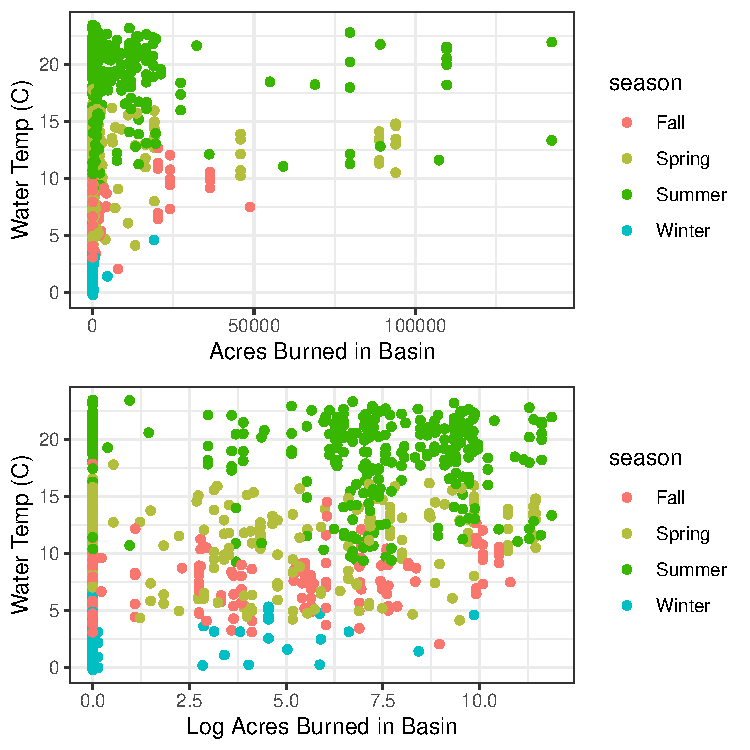
\includegraphics{D2P-Report_files/figure-latex/fig7-1.pdf}
\caption{\label{fig:figs7}Acres Burned by Wildfire and Water
Temperature}
\end{figure}

\begin{figure}
\centering
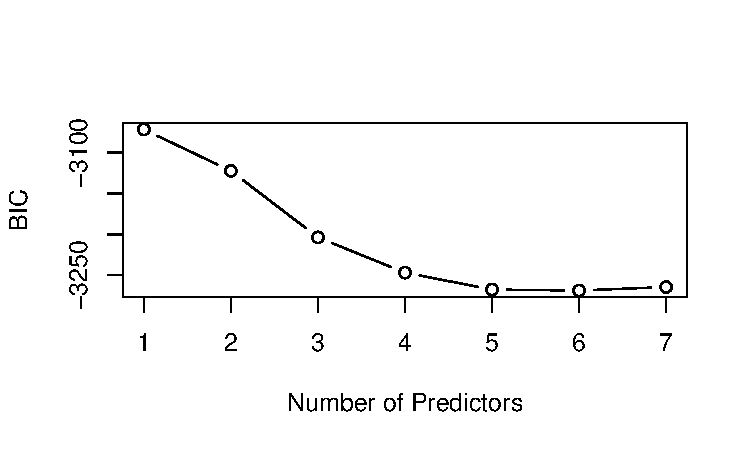
\includegraphics{D2P-Report_files/figure-latex/fig8-1.pdf}
\caption{\label{fig:figs8}Exhaustive Model Search - BIC}
\end{figure}

\begin{figure}
\centering
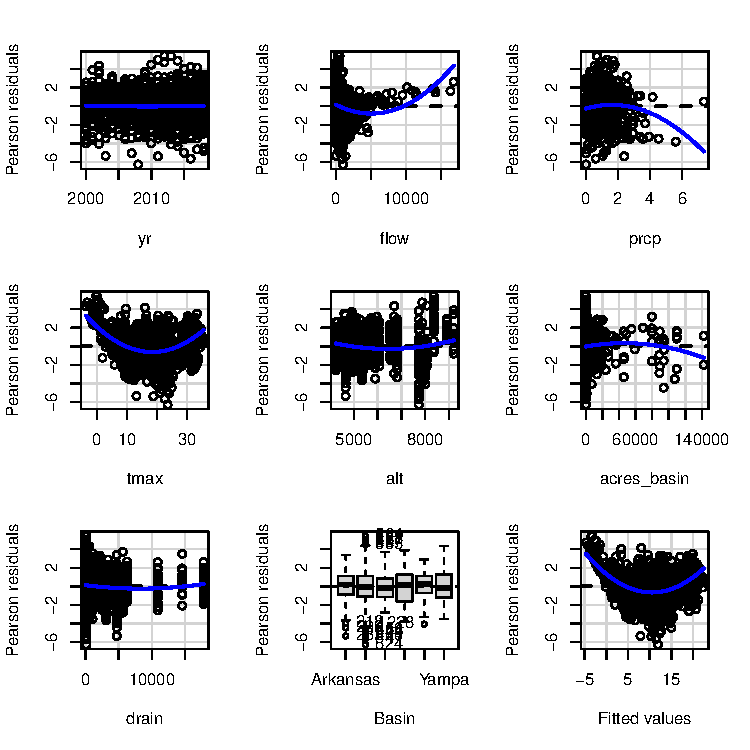
\includegraphics{D2P-Report_files/figure-latex/fig9-1.pdf}
\caption{\label{fig:figs9}Residual Plots - No Transformations}
\end{figure}

\begin{figure}
\centering
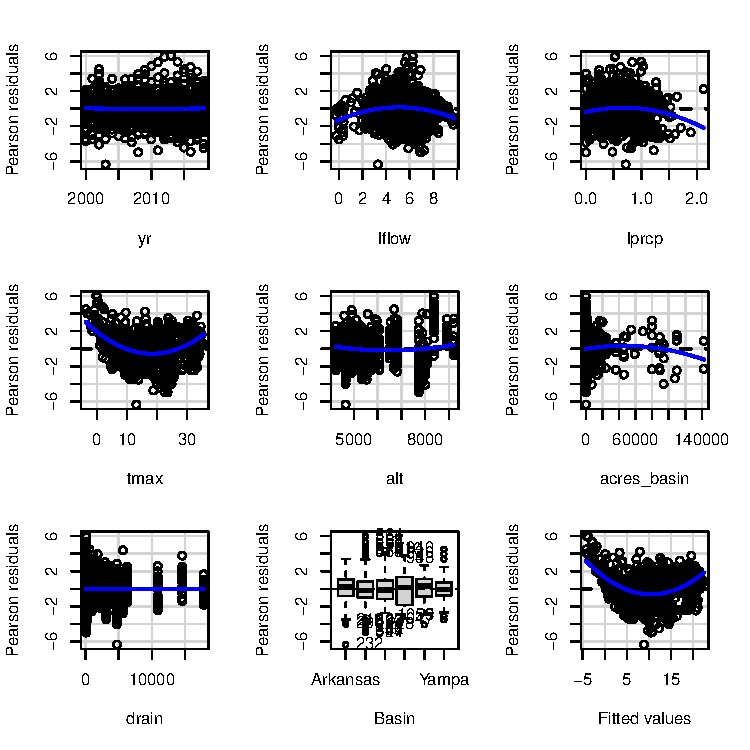
\includegraphics{D2P-Report_files/figure-latex/fig10-1.pdf}
\caption{\label{fig:figs10}Residual Plots - Log Transformations}
\end{figure}

\begin{figure}
\centering
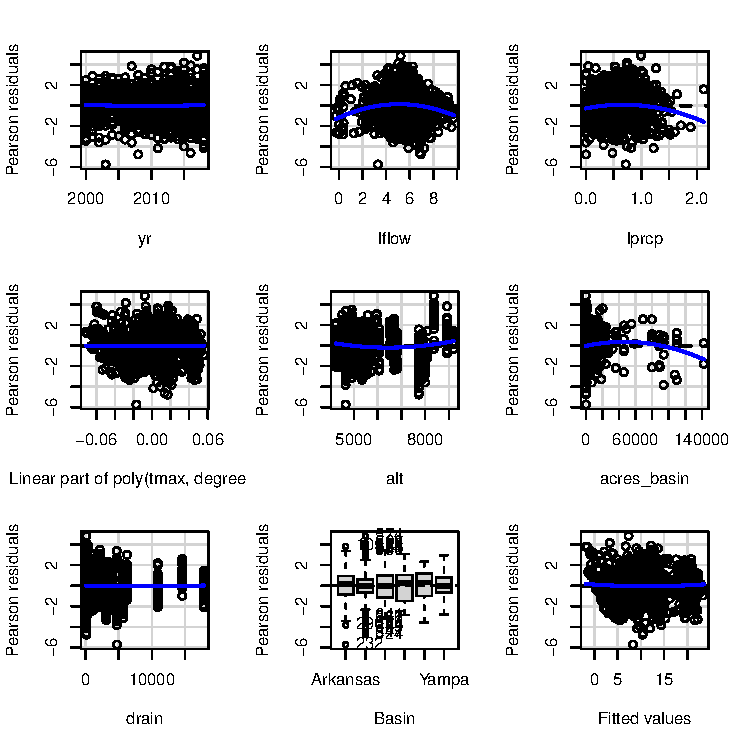
\includegraphics{D2P-Report_files/figure-latex/fig11-1.pdf}
\caption{\label{fig:figs11}Residual Plots - Quadratic Air Temp}
\end{figure}

\begin{figure}
\centering
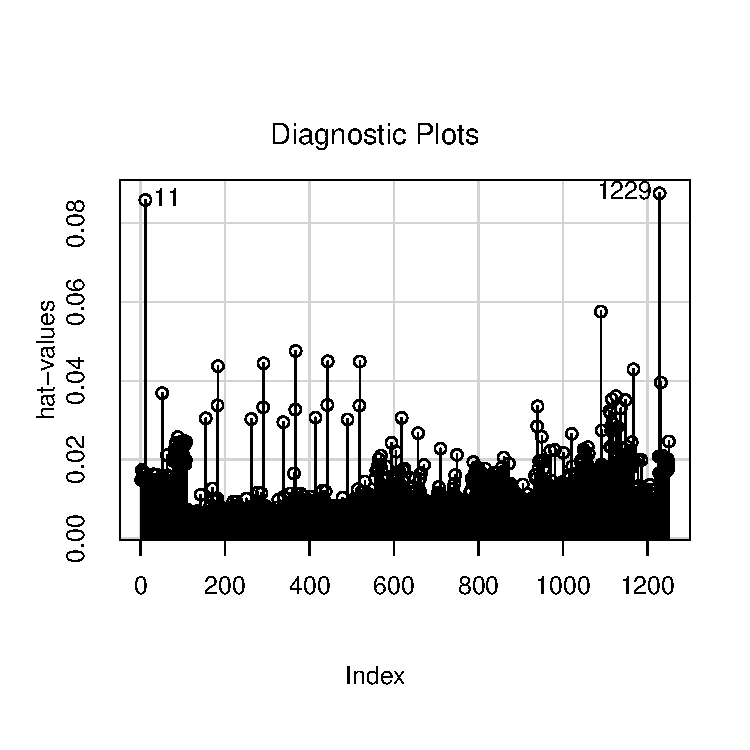
\includegraphics{D2P-Report_files/figure-latex/fig12-1.pdf}
\caption{\label{fig:figs12}Influence Index Plot}
\end{figure}

\begin{figure}
\centering
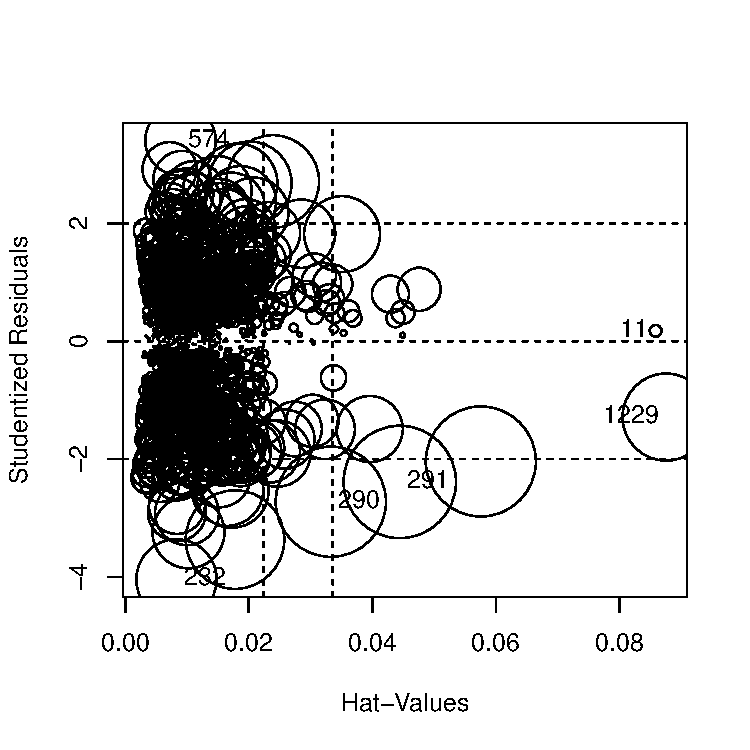
\includegraphics{D2P-Report_files/figure-latex/fig13-1.pdf}
\caption{\label{fig:figs13}Influence Plot}
\end{figure}

\begin{figure}
\centering
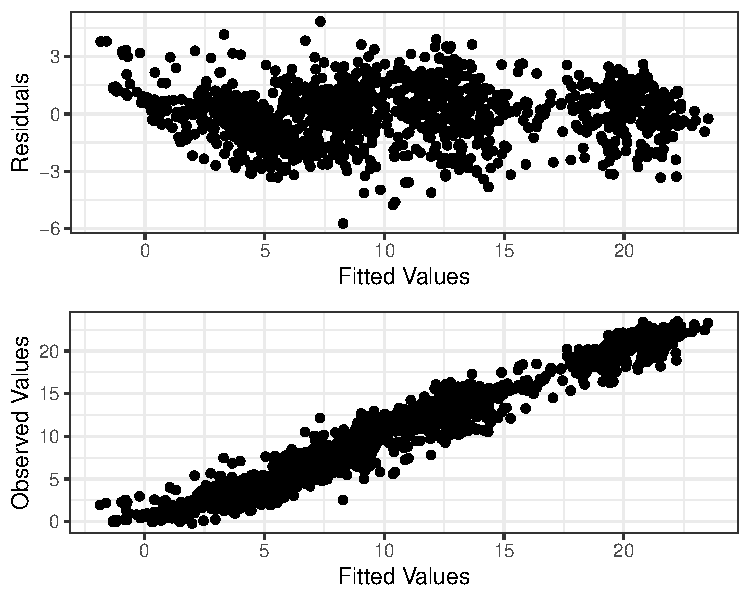
\includegraphics{D2P-Report_files/figure-latex/fig14-1.pdf}
\caption{\label{fig:figs14}Fitted Values versus Residuals \& Observed}
\end{figure}

\begin{figure}
\centering
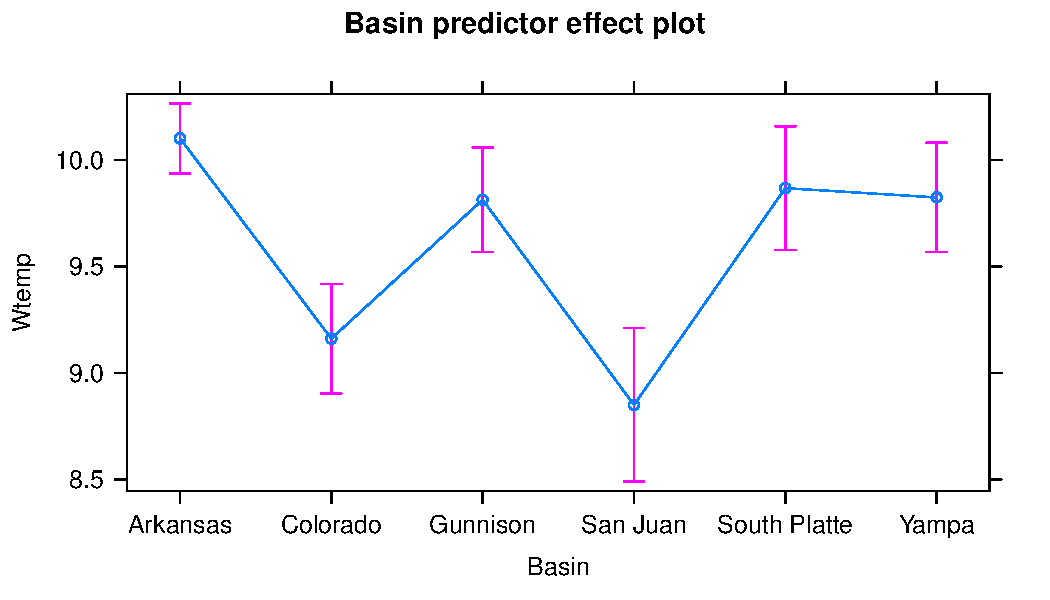
\includegraphics{D2P-Report_files/figure-latex/fig15-1.pdf}
\caption{\label{fig:figs15}Basin Effects Plots}
\end{figure}

\begin{figure}
\centering
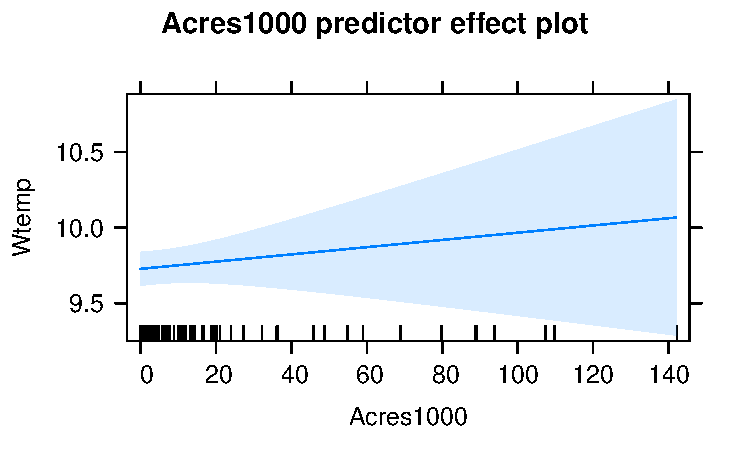
\includegraphics{D2P-Report_files/figure-latex/fig16-1.pdf}
\caption{\label{fig:figs16}Acres Burned Effects Plots}
\end{figure}

\end{document}
